\documentclass[11pt,a4paper]{article}
\usepackage[utf8]{inputenc}
\usepackage[T1]{fontenc}
\IfFileExists{lmodern.sty}{\usepackage{lmodern}}{}
\usepackage{amsmath,amssymb,amsthm,bm}
\usepackage{booktabs}
\usepackage{graphicx}
\usepackage[margin=2.5cm]{geometry}
\usepackage{hyperref}
\usepackage{listings}
\usepackage{xcolor}

\lstset{basicstyle=\ttfamily\small,columns=fullflexible,frame=single,
        backgroundcolor=\color{gray!6},breaklines=true,
        literate={Γ}{{$\Gamma$}}1}

\newtheorem{proposition}{Proposition}
\newcommand{\avg}[1]{\{\!\{#1\}\!\}}
\newcommand{\jump}[1]{[\![#1]\!]}
\newcommand{\qh}{\hat{\bm q}}
\newcommand{\q}{\bm q}

\title{A hybridized DG method with LMARS interface flux\\
for the linearized Euler equations with gravity,\\
with relaxed trace conditions and time integration without elimination}
\author{Documentation of \texttt{hdg\_relax\_euler\_gravity.py} / \texttt{HDGRelaxEuler.jl}}
\date{\today}

\begin{document}
\maketitle

\begin{abstract}
We describe a one-dimensional hybridized discontinuous Galerkin (HDG) discretization of the
compressible Euler equations with gravity, linearized about a hydrostatic background at rest.
The single-valued face traces are fixed by additional algebraic conditions (conservativity at
interior faces, reflection at walls). With the stabilization $\bm T=|\bm A|$ the resulting face
flux is exactly the linearized LMARS flux. Instead of eliminating the element unknowns in favour
of the traces (static condensation), the additional conditions are \emph{relaxed} into evolution
equations $\varepsilon\,\partial_t\qh = \bm H\q-\qh$, and the coupled element/trace system is
integrated in time directly, either monolithically with a stiffly accurate SDIRK method or with
an IMEX scheme whose implicit stage is local to each face. We prove well-balancing and discuss
conservation and the $\mathcal O(\varepsilon c/h)$ relaxation error, and report verification
results.
\end{abstract}

\tableofcontents

%=====================================================================
\section{Model}
%=====================================================================
Let $z$ be the vertical coordinate. The background state is at rest and in hydrostatic balance,
\begin{equation}
u_0=0,\qquad \partial_z p_0 = -\rho_0 g,\qquad c_0^2(z)=\gamma\frac{p_0}{\rho_0}=\gamma R T_0(z).
\end{equation}
The code uses a constant lapse rate $T_0(z)=T_{00}-\Gamma z$ (isothermal for $\Gamma=0$).
Linearizing the Euler equations around this state for perturbations $(\rho',u',p')$ gives
\begin{align}
\partial_t\rho' + \partial_z(\rho_0 u') &= 0,\\
\rho_0\partial_t u' + \partial_z p' &= -g\rho',\\
\partial_t p' + u'\,\partial_z p_0 + \gamma p_0\,\partial_z u' &= 0 .
\end{align}
With the momentum perturbation $m=\rho_0u'$ and the identity
$\partial_z(c_0^2 m)=\gamma\partial_z(p_0u') = \gamma p_0\partial_z u' + \gamma u'\partial_z p_0$
together with $\partial_z p_0=-\rho_0 g$, the pressure equation becomes
$\partial_t p' + \partial_z(c_0^2 m) = -(\gamma-1)g\,m$. Hence, with $\q=(\rho',m,p')^{\mathsf T}$,
\begin{equation}\label{eq:model}
\boxed{\;\partial_t\q + \partial_z\big(\bm A(z)\q\big) = \bm S\q,\qquad
\bm A=\begin{pmatrix}0&1&0\\0&0&1\\0&c_0^2&0\end{pmatrix},\quad
\bm S=\begin{pmatrix}0&0&0\\-g&0&0\\0&-(\gamma-1)g&0\end{pmatrix}.\;}
\end{equation}
The background density $\rho_0$ does not appear; only $c_0^2(z)$ does. The eigenvalues of $\bm A$
are $0,\pm c_0$. The zero-speed characteristic is pure $\rho'$ (right eigenvector $(1,0,0)^{\mathsf T}$),
and the acoustic part acts on $(m,p')$.

\paragraph{Hydrostatic perturbations.} Every state with $m=0$ and $\partial_z p'=-g\rho'$ is
steady. A scheme is called \emph{well-balanced} if it preserves the discrete analogue exactly.

%=====================================================================
\section{HDG discretization}
%=====================================================================
\subsection{Mesh, spaces, local problem}
The interval $[z_{\min},z_{\max}]$ is split into $N_e$ elements $K_e=[z_{e-1/2},z_{e+1/2}]$ of size
$h$. On each element $\q_h\in P_p(K_e)^3$, expanded in Legendre polynomials (modal basis, diagonal
mass matrix). On each face $f$ there is a single-valued trace $\qh_f\in\mathbb R^3$. The local
problem reads: for all $\bm v\in P_p(K)^3$,
\begin{equation}\label{eq:local}
(\bm v,\partial_t\q_h)_K = (\partial_z\bm v,\bm A\q_h)_K + (\bm v,\bm S\q_h)_K
 - \sum_{f\in\partial K}\bm v(z_f)^{\mathsf T}\,\widehat{\bm F}_{K,f},
\end{equation}
with the one-sided HDG flux ($n=\pm1$ the outward normal)
\begin{equation}\label{eq:hdgflux}
\widehat{\bm F}_{K,f} = \bm A(z_f)\,\qh_f\,n + \bm T_{K,f}\,\big(\q_h|_K(z_f)-\qh_f\big).
\end{equation}
The volume integrals are evaluated with $(p+3)$-point Gauss quadrature, which integrates
$(\partial_z\bm v, c_0^2 m)$ exactly for linear $c_0^2$.

\subsection{Additional (trace) conditions}
The traces are determined by algebraic conditions on each face.
\begin{itemize}
\item \textbf{Interior face} (left element $L$, right element $R$): conservativity,
\begin{equation}\label{eq:cons}
\widehat{\bm F}_{L,f}+\widehat{\bm F}_{R,f}=
\bm T_{L,f}(\q_L-\qh_f)+\bm T_{R,f}(\q_R-\qh_f)=\bm 0 .
\end{equation}
\item \textbf{Wall face} (reflecting): mirror average with the ghost state $(\rho',-m,p')$,
\begin{equation}\label{eq:wall}
\qh_f = \bm P\q_{\rm int},\qquad \bm P=\operatorname{diag}(1,0,1)\quad\Rightarrow\quad \hat m_f=0 .
\end{equation}
\end{itemize}
Both are written as $\qh = \bm H\q$, with $\bm H$ a sparse, face-local averaging operator.

\subsection{LMARS stabilization}
For the linear system the eigenvalues of $\bm A$ are $\{0,\pm c\}$, so
$|\bm A| = \bm A^2/c$, i.e.
\begin{equation}
\bm T_{\rm LMARS}(z_f) = |\bm A(z_f)| = \begin{pmatrix}0&0&1/c_f\\0&c_f&0\\0&0&c_f\end{pmatrix},
\qquad c_f=c_0(z_f).
\end{equation}
Because the background is continuous, $\bm T_{L,f}=\bm T_{R,f}$, and \eqref{eq:cons} gives
$|\bm A|(\q_L+\q_R-2\qh)=0$. The second and third rows give $\hat m=\avg{m}$ and
$\hat p=\avg{p'}$. The first column of $\bm A$ and of $|\bm A|$ vanishes, so $\hat\rho$ never
enters a flux and we set $\hat\rho=\avg{\rho'}$. Inserting $\qh=\avg{\q}$ into \eqref{eq:hdgflux}
(left side, $n=+1$, $\jump{\cdot}=(\cdot)_R-(\cdot)_L$):
\begin{equation}\label{eq:lmars}
\widehat{\bm F} = \begin{pmatrix} m^\ast\\ p^\ast\\ c_f^2 m^\ast\end{pmatrix},\qquad
m^\ast=\avg{m}-\frac{\jump{p'}}{2c_f},\qquad p^\ast=\avg{p'}-\frac{c_f}{2}\jump{m}.
\end{equation}
This is exactly the LMARS flux of Chen et al.~\cite{chen2013} linearized about $u_0=0$, with
interface velocity $u^\ast=m^\ast/\rho_0$ and interface pressure $p^\ast$. It is also the exact
Godunov flux of the acoustic subsystem. The flux identity is checked numerically in the code
(to round-off).

\paragraph{Alternative (LLF).} The option \texttt{flux="llf"} uses
$\bm T_K=c_K\operatorname{diag}(\tau_\rho,1,1)$ with an element value $c_K$, which gives a
$c_K$-weighted mean as the trace. With $\tau_\rho=0$ it is well-balanced, but $\rho'$ then
converges only at order $p$ (Table~\ref{tab:conv}). With $\tau_\rho>0$ it penalizes the
discontinuous $\rho'$ of a hydrostatic state, which destroys exact well-balancing. LMARS avoids
both problems: it penalizes only pressure and momentum jumps, and couples the mass flux to the
pressure jump.

\subsection{Matrix form}
Collecting all element coefficients in $\q\in\mathbb R^{n_q}$ ($n_q=3N_e(p+1)$) and all traces in
$\qh\in\mathbb R^{n_t}$ ($n_t=3N_f$), \eqref{eq:local}--\eqref{eq:wall} read
\begin{equation}\label{eq:dae}
\bm M\dot{\q} = \bm K\q+\bm G\qh,\qquad \bm 0 = \bm H\q-\qh ,
\end{equation}
where $\bm M$ is block diagonal (here diagonal), $\bm K$ contains the volume, source and element
parts of the penalty, $\bm G$ couples the traces into the element equations, and $\bm H$ is the
trace condition. The standard HDG implementation would eliminate $\q$ (static condensation) and
solve a global system for $\qh$ only. That is not done here.

%=====================================================================
\section{Relaxation of the additional conditions}
%=====================================================================
The algebraic condition is replaced by a relaxation equation with relaxation time $\varepsilon\ge0$:
\begin{equation}\label{eq:relax}
\boxed{\;
\begin{pmatrix}\bm M&\bm 0\\\bm 0&\varepsilon\bm I\end{pmatrix}
\frac{d}{dt}\begin{pmatrix}\q\\\qh\end{pmatrix}
=\underbrace{\begin{pmatrix}\bm K&\bm G\\\bm H&-\bm I\end{pmatrix}}_{\bm L}
\begin{pmatrix}\q\\\qh\end{pmatrix}.\;}
\end{equation}
For $\varepsilon=0$ this is the index-1 DAE \eqref{eq:dae}, i.e.\ the HDG/LMARS scheme. For
$\varepsilon>0$ the traces lag behind the element states. The system is integrated as a whole,
and no Schur complement is formed.

\paragraph{Relaxation error.} Expanding the slow manifold,
$\qh = \bm H\q - \varepsilon\,\bm H\dot\q + \mathcal O(\varepsilon^2)$. The trace defect enters
the element equations through $\bm G$, whose entries scale like $|\bm T|\sim c$, while
$\bm M\sim h$. The perturbation of the semi-discrete operator is therefore
\begin{equation}
\bm M^{-1}\bm G\,(\qh-\bm H\q) = \mathcal O\!\Big(\frac{c\,\varepsilon}{h}\Big)\,\dot{\q},
\end{equation}
i.e.\ a relative consistency error of order $\varepsilon c/h$. This scaling is confirmed by
Table~\ref{tab:eps}. To retain the HDG accuracy one needs $\varepsilon c/h \ll$ (spatial error),
e.g.\ $\varepsilon \lesssim 10^{-7}h/c$ for $p=3$ on the test mesh. The implicit or local
treatment of the relaxation term makes such small $\varepsilon$ affordable.

%=====================================================================
\section{Time integration without elimination}
%=====================================================================
\subsection{Monolithic SDIRK (\texttt{method="dirk"})}
We use the five-stage, fourth-order, L-stable and stiffly accurate SDIRK method of Hairer and
Wanner~\cite{hairer} with $a_{ii}=1/4$:
\[
\begin{array}{c|ccccc}
1/4 & 1/4\\ 3/4 & 1/2 & 1/4\\ 11/20 & 17/50 & -1/25 & 1/4\\
1/2 & 371/1360 & -137/2720 & 15/544 & 1/4\\
1 & 25/24 & -49/48 & 125/16 & -85/12 & 1/4\\\hline
 & 25/24 & -49/48 & 125/16 & -85/12 & 1/4
\end{array}
\]
With $\mathcal M=\operatorname{diag}(\bm M,\varepsilon\bm I)$, every stage solves
\begin{equation}
(\mathcal M-\Delta t\,a_{ii}\bm L)\,\bm Y_i = \mathcal M\bm U^n + \Delta t\sum_{j<i}a_{ij}\bm L\bm Y_j ,
\qquad \bm U^{n+1}=\bm Y_5 .
\end{equation}
The matrix $\mathcal M-\Delta t\,a_{ii}\bm L$ of the \emph{full} coupled system is factorized
once (sparse LU). It is regular for $\varepsilon=0$ as well, because its trace block is
$\Delta t\,a_{ii}\bm I$. Stiff accuracy makes the scheme valid for the DAE limit.

\subsection{IMEX ARS(2,2,2) (\texttt{method="imex"})}
The element part is treated explicitly and the relaxation implicitly, using ARS(2,2,2) of
Ascher, Ruuth and Spiteri~\cite{ars} with $\gamma=1-1/\sqrt2$ and $\delta=1-1/(2\gamma)$:
\[
\text{explicit: }
\begin{array}{c|ccc}0&0\\\gamma&\gamma&0\\1&\delta&1-\delta&0\\\hline&\delta&1-\delta&0\end{array}
\qquad
\text{implicit: }
\begin{array}{c|ccc}0&0\\\gamma&0&\gamma\\1&0&1-\gamma&\gamma\\\hline&0&1-\gamma&\gamma\end{array}
\]
Since the implicit right-hand side $(\bm H\q-\qh)/\varepsilon$ has no $\q$-component, each
implicit stage is solved \emph{pointwise per face}:
\begin{equation}
\qh^{(i)} = \frac{\qh^{\ast}+k\,\bm H\q^{(i)}}{1+k},\qquad k=\frac{\Delta t\,a^I_{ii}}{\varepsilon}.
\end{equation}
No linear system is solved at all. As $\varepsilon\to0$ this tends to $\qh^{(i)}=\bm H\q^{(i)}$,
i.e.\ the scheme is asymptotic preserving and reduces to an explicit HDG/LMARS (DG) scheme. The
time step is limited by the explicit CFL condition $\Delta t\lesssim h/(c(2p+1))$, and the
time accuracy is second order.

%=====================================================================
\section{Properties}
%=====================================================================
\begin{proposition}[Well-balancing]
Let $p'_h\in P_p$ be element-wise polynomial and globally continuous, $\rho'_h=-\partial_z p'_h/g$
element-wise, $m_h=0$, and $\qh=\bm H\q_h$. Then $\q_h$, $\qh$ are a steady state of
\eqref{eq:relax} for every $\varepsilon\ge0$, for both LMARS and LLF (with $\tau_\rho=0$).
\end{proposition}
\begin{proof}
Because $p'_h$ is continuous, $\hat p_f=p'_h(z_f)$ and $\hat m_f=0$, so $\bm H\q-\qh=0$ and the
trace equation is steady. In the flux \eqref{eq:hdgflux}, the $\rho'$-row is
$\hat m\,n+(p'_h-\hat p)/c=0$ and the $p'$-row is $c^2\hat m\,n+c(p'_h-\hat p)=0$. The
$\rho'$-jump enters neither, because the first columns of $\bm A$ and $\bm T$ vanish. Both volume
terms of the $\rho'$ and $p'$ equations vanish since $m_h=0$. The $m$-row of the flux is
$\hat p\,n+c(m-\hat m)=p'_h(z_f)\,n$, and integrating by parts,
$(\partial_z v,p'_h)_K-[v\,p'_h]_{\partial K}-g(v,\rho'_h)_K = -(v,\partial_zp'_h+g\rho'_h)_K=0$.
\end{proof}

\paragraph{Conservation.} The total mass changes by the sum of the two one-sided mass fluxes on
each face. For LMARS this sum is $(2/c_f)(\avg{p'}-\hat p)=(2/c_f)\,\varepsilon\,\dot{\hat p}$:
mass is conserved to round-off for $\varepsilon=0$, with an $\mathcal O(\varepsilon)$ drift
otherwise (Table~\ref{tab:wall}). The same holds for $m$ and $p'$. With LLF and $\tau_\rho=0$
the mass flux is $\hat m$, which is single-valued, so mass is conserved exactly for every
$\varepsilon$, but $\rho'$ loses one order of accuracy.

\paragraph{Stability.} For walls and $\varepsilon=0$ the largest real part of the spectrum of the
semi-discrete operator is $\approx 5\cdot10^{-15}$ (lapse-rate atmosphere, $N_e=16$, $p=2$). With
$\varepsilon>0$ no eigenvalue with positive real part beyond the physical growth of the periodic
normal mode was observed.

%=====================================================================
\section{Verification}
%=====================================================================
All numbers below come from the Python implementation (\texttt{run\_tests.py}). The Julia port
implements the same algorithm and should reproduce them to 3--4 significant digits.

\subsection{Convergence}
Periodic domain $[0,2000]$\,m, isothermal atmosphere ($T_0=250$\,K), exact normal mode
$\q=\Re(\bm v e^{ikz+\lambda t})$ of \eqref{eq:model} on the upward acoustic branch, amplitude
$100$\,Pa, run for one acoustic transit. The SDIRK step is $\Delta t=h/(c(2p+1))$.

\begin{table}[h]\centering
\caption{$L^2$ error in $p'$ and observed rates (last refinement), $N_e=8,16,32,64$.}\label{tab:conv}
\begin{tabular}{llcccccc}\toprule
flux / method & $p$ & $N_e=8$ & $16$ & $32$ & $64$ & rate $p'$ & rate $\rho'$\\\midrule
LMARS, DIRK, $\varepsilon=0$ & 1 & 1.89e+2 & 3.83e+1 & 8.80e+0 & 2.15e+0 & 2.04 & 2.04\\
 & 2 & 8.59e+0 & 1.07e+0 & 1.34e-1 & 1.70e-2 & 3.00 & 3.00\\
 & 3 & 4.09e-1 & 2.59e-2 & 1.62e-3 & 1.01e-4 & 4.00 & 4.00\\
LMARS, DIRK, $\varepsilon=10^{-9}h/c$ & 3 & 4.09e-1 & 2.59e-2 & 1.62e-3 & 1.11e-4 & 3.86 & 3.86\\
LMARS, IMEX, $\varepsilon=10^{-9}h/c$ & 2 & 9.39e+0 & 1.42e+0 & 2.70e-1 & 6.10e-2 & 2.15 & 2.15\\
LLF ($\tau_\rho=0$), DIRK, $\varepsilon=0$ & 1 & 1.88e+2 & 3.82e+1 & 8.79e+0 & 2.15e+0 & 2.04 & 1.00\\
 & 3 & 4.09e-1 & 2.58e-2 & 1.62e-3 & 1.01e-4 & 4.00 & 3.00\\\bottomrule
\end{tabular}
\end{table}
LMARS gives the optimal order $p+1$ in all components. The IMEX result for $p=2$ is limited by
the second-order time integrator.

\subsection{Relaxation error}
\begin{table}[h]\centering
\caption{$L^2$ error in $p'$ versus $\varepsilon c/h$ ($N_e=16$, $p=3$); the $\varepsilon=0$
reference is $2.586\cdot10^{-2}$.}\label{tab:eps}
\begin{tabular}{lccccccc}\toprule
$\varepsilon c/h$ & $10^{-8}$ & $10^{-7}$ & $10^{-6}$ & $10^{-5}$ & $10^{-4}$ & $10^{-3}$ & $10^{-2}$\\\midrule
DIRK & 2.59e-2 & 2.63e-2 & 5.26e-2 & 4.57e-1 & 4.56e+0 & 4.55e+1 & 4.46e+2\\
IMEX & 4.79e-1 & 4.75e-1 & 4.34e-1 & 4.00e-2 & 4.08e+0 & 4.50e+1 & 4.45e+2\\\bottomrule
\end{tabular}
\end{table}
The error grows linearly in $\varepsilon c/h$ once it exceeds the discretization error. The IMEX
floor is the second-order time error.

\subsection{Well-balancing}
Lapse-rate atmosphere ($T_0=288$\,K, $\Gamma=6.5$\,K/km), walls, $[0,10]$\,km, $N_e=40$, $p=3$.
The hydrostatic perturbation is $p'$ = continuous interpolant of
$50\cos(2\pi z/7\,\mathrm{km})+30(z/10\,\mathrm{km})^2$\,Pa, with $\rho'=-\partial_zp'/g$. After 200 steps
the maximum relative deviation is $3.7\cdot10^{-12}$ (DIRK, $\varepsilon=0$ and $10^{-3}$) and
$\le10^{-15}$ (IMEX), i.e.\ round-off.

\subsection{Acoustic pulse between walls}
Same atmosphere, $N_e=80$, $p=3$, Gaussian pressure pulse ($100$\,Pa, width $300$\,m, centred at
$3$\,km), $t\in[0,40]$\,s.
\begin{table}[h]\centering
\caption{Mass drift and trace residual $\max|\bm H\q-\qh|$, LMARS.}\label{tab:wall}
\begin{tabular}{lcc}\toprule
case & $\max|\Delta \text{mass}|$ & trace residual\\\midrule
HDG $\varepsilon=0$ (DIRK) & 4.0e-14 & 4.3e-12\\
$\varepsilon=10^{-4}h/c$ (DIRK) & 1.1e-5 & 4.1e-3\\
$\varepsilon=10^{-4}h/c$ (IMEX) & 1.1e-5 & 4.1e-3\\
$\varepsilon=10^{-2}h/c$ (DIRK) & 1.1e-3 & 4.0e-1\\\bottomrule
\end{tabular}
\end{table}

\IfFileExists{convergence.png}{%
\begin{figure}[h]\centering
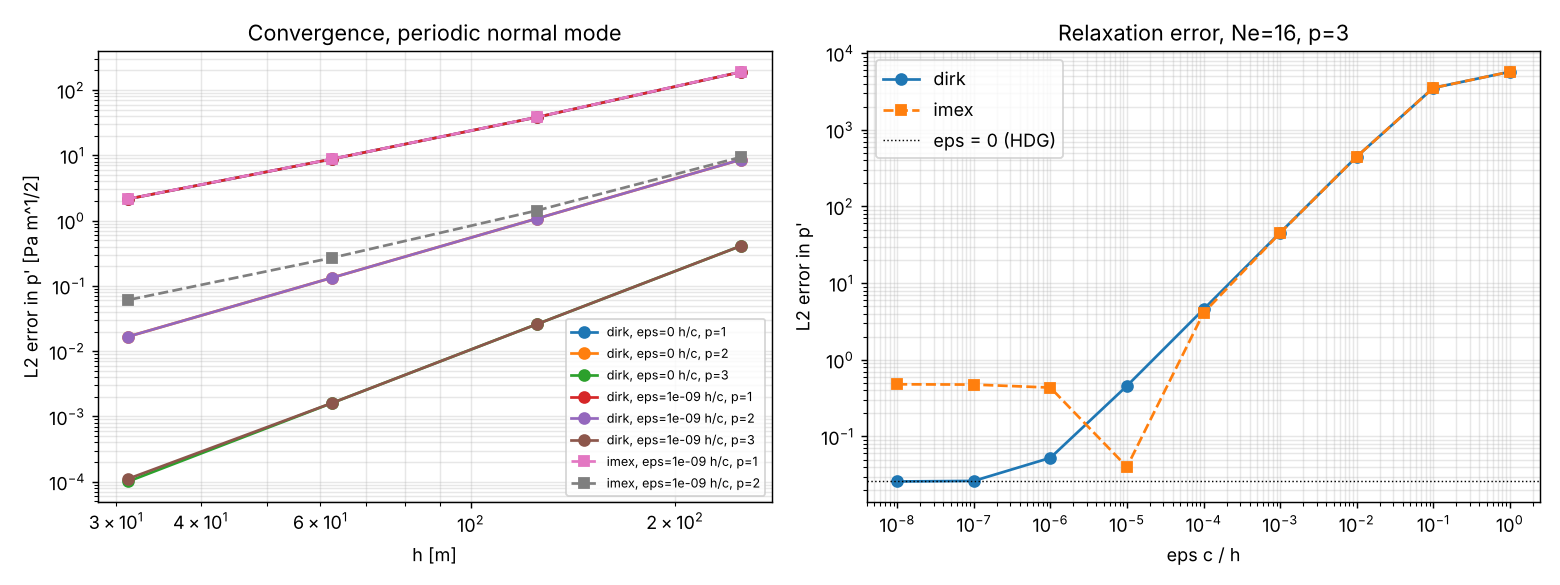
\includegraphics[width=\textwidth]{convergence.png}
\caption{Left: convergence for the normal mode. Right: relaxation error versus $\varepsilon c/h$.}
\end{figure}}{}
\IfFileExists{wall_demo.png}{%
\begin{figure}[h]\centering
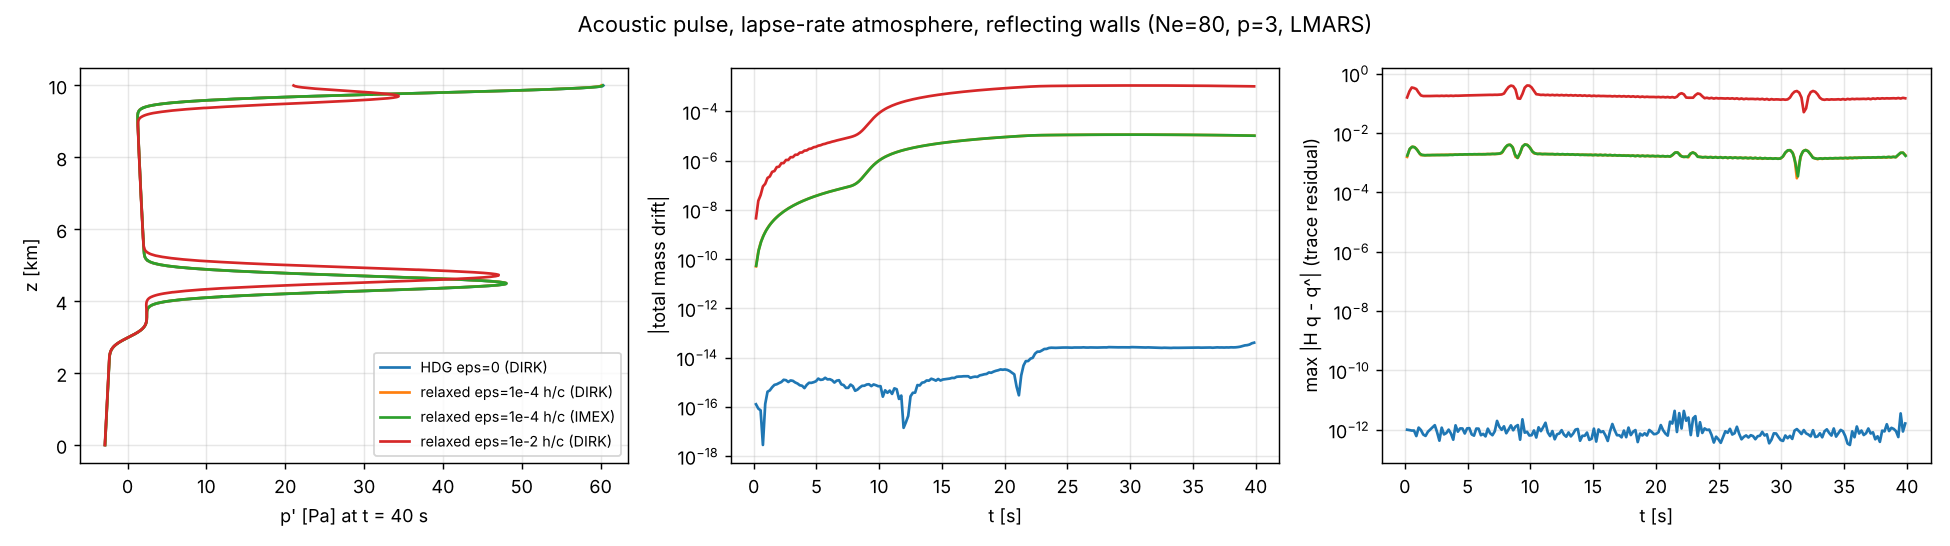
\includegraphics[width=\textwidth]{wall_demo.png}
\caption{Acoustic pulse with walls: pressure at $t=40$\,s, mass drift, trace residual.}
\end{figure}}{}

%=====================================================================
\section{Code}
%=====================================================================
\subsection{Files}
\begin{tabular}{ll}
\texttt{hdg\_relax\_euler\_gravity.py} & Python solver (NumPy/SciPy)\\
\texttt{run\_tests.py} & Python tests and plots\\
\texttt{julia/HDGRelaxEuler.jl} & Julia module (standard library only)\\
\texttt{julia/run\_tests.jl} & Julia tests, writes CSV files\\
\texttt{julia/plot\_results.jl} & optional plots (needs \texttt{Plots.jl})\\
\end{tabular}

\subsection{Data layout}
Element coefficient $(e,r,i)$ (element, variable $\rho',m,p'$, Legendre mode) is stored at
$((e-1)\cdot3+(r-1))(p+1)+i$ (Julia, 1-based) or $(3e+r)(p+1)+i$ (Python, 0-based). Trace
$(f,r)$ is stored at $3(f-1)+r$ (Julia) or $3f+r$ (Python). The state vector is $\bm U=(\q,\qh)$.

\subsection{Usage (Julia)}
\begin{lstlisting}[language=Python]
include("HDGRelaxEuler.jl"); using .HDGRelaxEuler
atm = Atmosphere(T0 = 288.0, Γ = 0.0065)
s   = HDGRelax(80, 3, 0.0, 1.0e4, atm; bc = :wall, flux = :lmars, eps = 0.0)
q0  = project(s, z -> vcat(0 .* z', 0 .* z', (100 .* exp.(-((z .- 3000) ./ 300) .^ 2))'))
U0  = initial_state(s, q0)                    # traces consistent: qhat = H q
U   = run!(s, U0, 1e-3, 1000; method = :dirk) # or :imex
z, Q = evaluate(s, U[1:s.nq])                 # Q[3,:] = p'
\end{lstlisting}
The Python API is the same: \texttt{HDGRelax(Ne, p, zmin, zmax, atm, bc="wall", eps=0.0,
flux="lmars")}, \texttt{s.run(U0, dt, n, method="dirk")}.

\subsection{Main options}
\begin{tabular}{lll}\toprule
option & values & meaning\\\midrule
\texttt{bc} & wall / periodic & reflecting walls (\eqref{eq:wall}) or periodic\\
\texttt{flux} & lmars / llf & stabilization $\bm T$\\
\texttt{eps} & $\ge 0$ & relaxation time $\varepsilon$ (seconds)\\
\texttt{tau\_scale} & $>0$ & multiplies $\bm T$\\
\texttt{tau\_rho} & $\ge0$ & $\rho'$ penalty weight (LLF only)\\
\texttt{method} & dirk / imex & monolithic SDIRK4 / local IMEX ARS(2,2,2)\\\bottomrule
\end{tabular}

\begin{thebibliography}{9}
\bibitem{chen2013} X.~Chen, N.~Andronova, B.~van Leer, J.~E.~Penner, J.~P.~Boyd, C.~Jablonowski,
S.-J.~Lin, A control-volume model of the compressible Euler equations with a vertical Lagrangian
coordinate, \emph{Mon.\ Wea.\ Rev.} 141 (2013) 2526--2544.
\bibitem{cockburn2009} B.~Cockburn, J.~Gopalakrishnan, R.~Lazarov, Unified hybridization of
discontinuous Galerkin, mixed, and continuous Galerkin methods for second order elliptic
problems, \emph{SIAM J.\ Numer.\ Anal.} 47 (2009) 1319--1365.
\bibitem{ars} U.~M.~Ascher, S.~J.~Ruuth, R.~J.~Spiteri, Implicit-explicit Runge--Kutta methods for
time-dependent partial differential equations, \emph{Appl.\ Numer.\ Math.} 25 (1997) 151--167.
\bibitem{hairer} E.~Hairer, G.~Wanner, \emph{Solving Ordinary Differential Equations II: Stiff and
Differential-Algebraic Problems}, 2nd ed., Springer, 1996.
\bibitem{jinxin} S.~Jin, Z.~Xin, The relaxation schemes for systems of conservation laws in
arbitrary space dimensions, \emph{Comm.\ Pure Appl.\ Math.} 48 (1995) 235--276.
\end{thebibliography}
\end{document}
